\section{MoogleServer}
\begin{frame}[fragile]{MoogleServer}
\begin{center}
  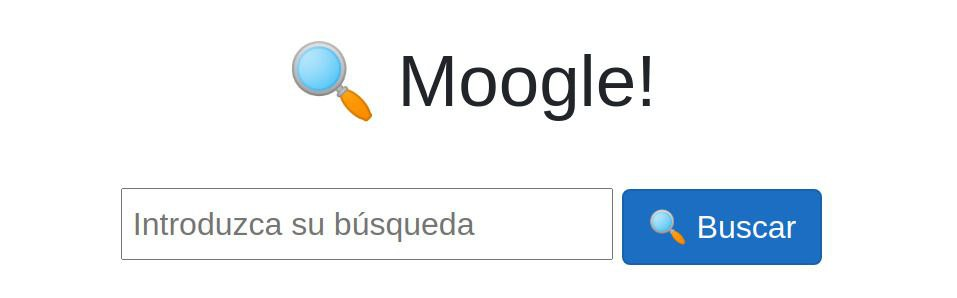
\includegraphics[width=8cm]{moogle.jpg}
\end{center}

MoogleServer es la biblioteca gr\'afica del proyecto escrita en lenguaje web html,css,javaScript, aunque 
es bastante pobre y sencilla para cualquier usuario de la red. Contiene una barra de b\'usqueda en la cual
se deber\'a escribir lo que se necesita buscar y a su lado un bot\'on de "Buscar" para ejecutar la misma.
Sobre el fondo blanco se mostrar\'an los datos de la b\'usqueda.

\end{frame}